\newpage
IRSTI 65.59.15
\hfill {\bfseries \href{https://doi.org/10.58805/kazutb.v.3.24-510}{https://doi.org/10.58805/kazutb.v.3.24-510}}

\sectionwithauthors{K. Makangali, G. Ospankulova, G.Tokysheva}{ENHANCING QUALITY AND SHELF LIFE OF ORGANIC SAUSAGES WITH
PURSLANE POWDER}
\begin{center}

{\bfseries K. Makangali\envelope,} {\bfseries G. Ospankulova, G.
Tokysheva}

NJSC «S.Seifullin Kazakh agrotechnical research University», Astana,
Kazakhstan
\end{center}

\envelope Corresponding author: kmakangali@mail.ru \vspace{0.5cm}

This study investigates the effects of adding purslane powder (Portulaca
oleracea) to organic sausages made from organic beef, focusing on
physicochemical properties, sensory characteristics, and microbiologi-cal
stability. The use of natural additives is crucial in organic sausage
production due to restrictions on synthetic preservatives and sodium
nitrite. Samples were prepared with 0.8\%, 1.2\%, and 1.4\% purslane
powder and compared to a control without purslane. Results showed that
purslane powder significantly improved moisture retention, with the
highest levels observed in the 1.2\% and 1.4\% samples. pH values
remained stable across all samples, indicating effective acidity
regulation. Water activity (aw) values were consistent, ensuring
microbiological safety. The total viable count (TVC) was significantly
lower in samples with purslane, particularly at 1.2\% and 1.4\%
concentrations, compared to the control. Sensory analysis indicated that
the sample with 1.2\% purslane maintained high scores similar to the
control, while the 1.4\% sample exhibited a bitter taste and greenish
tint, negatively affecting its sensory attributes. The use of organic
beef aligns with consumer demand for natural and healthy products,
providing high-quality protein without synthetic additives. Purslane
powder, known for its antioxidant and antimicrobial properties, proved
to be an effective natural additive for improving the quality and shelf
life of organic sausages. The optimal concentration of 1.2\% purslane is
recommended, offering a balance between enhan-ced physicochemical
properties and favorable sensory characteristics. This study supports
the use of natural additives in organic meat products, promoting
healthier and more sustainable food options.

{\bfseries Keywords:} organic sausages, purslane powder, physicochemical
properties, sensory analysis, micro-biological stability, natural
additives.

\sectionheading{УЛУЧШЕНИЕ КАЧЕСТВА И СРОКА ГОДНОСТИ ОРГАНИЧЕСКИХ КОЛБАС С
ПОМОЩЬЮ ПОРОШКА ПОРТУЛАКА}
\begin{center}

{\bfseries К.К. Макангали\envelope, Г.Х. Оспанкулова, Г.М.
Токышева}

НАО «Казахский агротехнический исследовательский университет
им.С.Сейфуллина», Астана, Казахстан,

e-mail: kmakangali@mail.ru
\end{center}

Исследование изучает влияние добавления порошка портулака (Portulaca
oleracea) в органические колбасы, изготовленные из органической
говядины, с акцентом на физико-химические свойства, сенсорные
характеристики и микробиологическую стабильность. Использование
натуральных добавок имеет решающее значение в производстве органических
колбас из-за ограничений на синтетические консерванты и нитрит натрия.
Были подготовлены образцы с 0,8\%, 1,2\% и 1,4\% порошка портулака и
сравнены с контрольным образцом без портулака. Результаты показали, что
порошок портулака значительно улучшил удержание влаги, при этом самые
высокие уровни наблюдались в образцах с 1,2\% и 1,4\%. Значения pH
оставались стабильными во всех образцах, что указывает на эффективное
регулирование кислотности. Значения активности воды (aw) были
постоянными, что обеспечивало микробиологическую безопасность. Общее
количество жизнеспособных бактерий (КМАФАнМ) бы-ло значительно ниже в
образцах с портулаком, особенно при концентрациях 1,2\% и 1,4\%, по
сравне-нию с контрольным образцом. Сенсорный анализ показал, что образец
с 1,2\% портулака сохранял высокие оценки, аналогичные контрольному,
тогда как образец с 1,4\% портулака имел горький вкус и зеленоватый
оттенок, что отрицательно сказалось на его сенсорных характеристиках.
Использование органической говядины соответствует потребительскому
спросу на натуральные и полезные продукты, обеспечивая
высококачественный белок без синтетических добавок. Порошок портулака,
известный своими антиоксидантными и антимикробными свойствами, оказался
эффективной натуральной добавкой для улучшения качества и срока годности
органических колбас. Рекомендуется оптимальная концентрация 1,2\%
портулака, обеспечивающая баланс между улучшенными физико-химическими
свойствами и благоприятными сенсорными характеристиками. Это
исследование под-держивает использование натуральных добавок в
органических мясных продуктах, способствуя продвижению более здоровых и
устойчивых вариантов питания.

{\bfseries Ключевые слова:} органические колбасы, порошок портулака,
физико-химические свойства, сен-сорный анализ, микробиологическая
стабильность, натуральные добавки.

\sectionheading{ПОРТУЛАК ҰНТАҒЫ ҚОСЫЛҒАН ОРГАНИКАЛЫҚ ШҰЖЫҚТАРДЫҢ САПАСЫ МЕН
САҚТАУ МЕРЗІМІН ЖАҚСАРТУ}
\begin{center}

{\bfseries Қ.Қ. Мақанғали\envelope, Г.Х. Оспанкулова, Г.М.
Тоқышева}

«С.Сейфуллина атындағы Қазақ агротехникалық зерттеу университеті» КеАҚ,
Астана, Қазақстан,

e-mail: kmakangali@mail.ru
\end{center}

Зерттеу физикалық-химиялық қасиеттерге, сенсорлық сипаттамаларға және
микробиологиялық тұрақтылыққа назар аудара отырып, органикалық сиыр
етінен жасалған органикалық шұжықтарға портулак ұнтағын (Portulaca
oleracea) қосудың әсерін зерттейді. Табиғи қоспаларды қолдану
синтети-калық консерванттар мен натрий нитритіне шектеулерге байланысты
органикалық шұжық өндірісін-де өте маңызды. Үлгілер 0,8\%, 1,2\% және
1,4\% портулак ұнтағымен дайындалды және портулаксыз бақылаумен
салыстырылды. Нәтижелер портулак ұнтағы ылғалдың сақталуын айтарлықтай
жақсарт-қанын көрсетті, ең жоғары деңгейлер 1,2\% және 1,4\% үлгілерде
байқалды. рH мәндері барлық үлгі-лерде тұрақты болып қалды, бұл
қышқылдықтың тиімді реттелуін көрсетеді. Су белсенділігінің (aw)
көрсеткіштері микробиологиялық қауіпсіздікті қамтамасыз ете отырып,
сәйкес болды. Жалпы өміршеңдік көрсеткіші (TVC) портулак сынамаларында
айтарлықтай төмен болды, әсіресе бақылаумен салыстырғанда 1,2\% және
1,4\% концентрацияда. Сенсорлық талдау көрсеткендей, 1,2\% портулак
сынамасы бақылауға ұқсас жоғары балл жинады, ал 1,4\% сынамада ащы дәм
мен жасыл реңк байқалды, бұл оның сенсорлық қасиеттеріне теріс әсер
етті. Органикалық сиыр етін пайдалану тұтынушылардың табиғи және пайдалы
өнімдерге деген сұранысына сәйкес келеді, синтетикалық қоспаларсыз
жоғары сапалы ақуызды қамтамасыз етеді. Антиоксиданттық және микробқа
қарсы қасиеттерімен танымал портулак ұнтағы органикалық шұжықтардың
сапасы мен сақтау мерзімін жақсарту үшін тиімді табиғи қоспа болып
шықты. Жақсартылған физика-химиялық қасиеттері мен қолайлы сенсорлық
сипаттамалары арасындағы тепе-теңдікті қамтамасыз ететін 1,2\%
портулактың оңтайлы концентрациясы ұсынылады. Бұл зерттеу органикалық ет
өнімдерінде табиғи қоспаларды қолдануды қолдайды, бұл тағамның пайдалы
және тұрақты нұсқаларын жасауға ықпал етеді.

{\bfseries Түйін сөздер:} органикалық шұжықтар, портулак ұнтағы,
физика-химиялық қасиеттері, сенсор-лық анализі, микробиологиялық
тұрақтылығы, табиғи қоспалары.
\begin{multicols}{2}

{\bfseries Introduction.} In recent years, the interest in organic food
products has significantly increased due to their presumed health
benefits and lower environmental impact. One of the promising directions
in the organic production of meat products is the use of natural
additives, such as plant extracts and powders, to improve the quality
and safety of the products. In this context, purslane powder (Portulaca
oleracea) is of particular interest, as it possesses a range of
beneficial properties, including antioxidant and antimicrobial activity
{[}1{]}.

The global market for organic food has been experiencing steady growth,
driven by consumer awareness and demand for healthier and more
environmentally friendly food options. According to recent reports, the
market for organic products is projected to continue expanding, with
significant investments being made in research and development of
organic farming and production techniques {[}2, 3{]}.

Natural additives have gained considerable attention in the food
industry due to their potential to enhance food quality and safety.
Plant-based extracts and powders, in particular, are being extensively
studied for their bioactive compounds that can act as natural
preservatives and health enhancers. Studies have shown that these
natural additives can improve the sensory attributes of food, extend
shelf life, and reduce the need for synthetic additives {[}4,5{]}.

Purslane (Portulaca oleracea) is a succulent plant widely recognized for
its nutritional and medicinal properties. It is rich in omega-3 fatty
acids, vitamins, minerals, and bioactive compounds such as phenolics and
flavonoids. Previous research has highlighted its antioxidant
properties, which can help in preventing oxidative deterioration of food
products. Moreover, its antimicrobial activity has been reported to
inhibit the growth of various foodborne pathogens, making it a promising
natural additive for food preservation {[}6,7{]}.

Water activity (aw) is a crucial parameter in determining the shelf life
and safety of food products. It measures the availability of free water
for microbial growth and chemical reactions. High water activity in food
can lead to the proliferation of spoilage and pathogenic microorganisms,
which adversely affects the product\textquotesingle s quality and
safety. Therefore, controlling water activity is essential in the
production of meat products, especially organic ones, to ensure their
microbiological stability and extend their shelf life {[}8,9{]}.

The use of natural additives like purslane powder in meat products can
potentially regulate water activity and enhance antimicrobial
properties. Purslane contains phenolic compounds and flavonoids that
exhibit significant antimicrobial potential, which can contribute to
maintaining the microbiological quality of the product {[}10{]}.

The aim of this study is to comprehensively evaluate the effect of
purslane powder on water activity and antimicrobial activity in organic
sausages. The determination of the influence of different concentrations
of purslane powder on water activity (aw) in organic sausages was
measured using the AquaLab 4TE analyzer (METER Group, USA) to ensure
accuracy and reliability of the results. The analysis of changes in
physicochemical indicators (moisture, pH) and their impact on the
microbiological stability of the products during storage was conducted.
The moisture content and pH in sausage samples with added purslane
powder were analyzed (Tango-R FT-NIR spectrometer, Bruker, Germany), as
well as their changes during storage (Table 1).

{\bfseries Materials and methods.} Moisture Content and pH Measurement. The
moisture content and pH of the sausage samples were determined using the
Tango-R FT-NIR spectrometer (Bruker, Germany). Approximately 10 grams of
each sausage sample were homogenized, and the homogenate was analyzed
using the FT-NIR spectrometer. This technique allows for rapid and
non-destructive analysis of moisture and pH by measuring the
near-infrared absorption spectra of the samples. The instrument was
calibrated using standard reference materials to ensure accuracy. The
moisture content and pH values were obtained from the spectral data
using the instrument\textquotesingle s software.

Water Activity (aw) Measurement. Water activity (aw) of the sausage
samples was measured using the AquaLab 4TE water activity meter (METER
Group, USA). Approximately 2 grams of each sample were placed in the
sample cup, ensuring that the sample surface was level and free from air
pockets. The sample cup was then placed in the measurement chamber of
the AquaLab, and the aw value was recorded once the reading stabilized.
The instrument was calibrated regularly using standard calibration salts
(aw 0.760 and aw 0.920) to ensure accuracy and reliability of the
results.

Antimicrobial Activity Analysis. To evaluate the antimicrobial activity
of the purslane powder in the sausage samples, microbiological analysis
was conducted. The total viable count (TVC) was assessed using Compact
Dry plates (Nissui Pharmaceutical Co., Ltd., Japan). Sausage samples
were homogenized in sterile saline solution and serially diluted. An
aliquot (1 ml) of the diluted sample was applied to the Compact Dry
plate and spread evenly. The plates were incubated at 35°C for 48 hours,
after which the colony-forming units (CFU) were counted. The results
were expressed as log CFU per gram of sausage.

Statistical Analysis. All experiments were conducted in triplicate, and
the results were expressed as mean ± standard deviation. Statistical
analysis was performed using ANOVA (Analysis of Variance) to determine
the significance of differences between the control and experimental
samples. A p-value of less than 0.05 was considered statistically
significant.

{\bfseries Results and discussion.} The moisture content of the sausage
samples showed a general decrease over the storage period for both the
control and experimental samples. However, the experimental samples with
purslane powder exhibited higher moisture retention compared to the
control. For instance, at 9 days, the control sample had a moisture
content of 54.9\%, whereas the samples with 0.8\%, 1.2\%, and 1.4\%
purslane powder had moisture contents of 57.2\%, 58.7\%, and 58.9\%,
respectively. This suggests that the addition of purslane powder helps
in retaining moisture in the sausages, which could be beneficial for the
texture and juiciness of the product (table 1).
\end{multicols}


\begin{longtable}[]{|@{}
  >{\raggedright\arraybackslash}p{(\columnwidth - 10\tabcolsep) * \real{0.1524}}|
  >{\raggedright\arraybackslash}p{(\columnwidth - 10\tabcolsep) * \real{0.1221}}|
  >{\raggedright\arraybackslash}p{(\columnwidth - 10\tabcolsep) * \real{0.1892}}|
  >{\raggedright\arraybackslash}p{(\columnwidth - 10\tabcolsep) * \real{0.1787}}|
  >{\raggedright\arraybackslash}p{(\columnwidth - 10\tabcolsep) * \real{0.1787}}|
  >{\raggedright\arraybackslash}p{(\columnwidth - 10\tabcolsep) * \real{0.1787}}@{}|}
  
\caption*{Table 1 - Physicochemical parameters of control and experimental
 sausage samples with added purslane powder} \\
\hline
% \toprule
\begin{minipage}[b]{\linewidth}\raggedright
Parameter
\end{minipage} & \begin{minipage}[b]{\linewidth}\raggedright
Storage, days
\end{minipage} & \begin{minipage}[b]{\linewidth}\raggedright
Control
\end{minipage} & \begin{minipage}[b]{\linewidth}\raggedright
Experiment 1 (0.8\% purslane)
\end{minipage} & \begin{minipage}[b]{\linewidth}\raggedright
Experiment 2 (1.2\% purslane)
\end{minipage} & \begin{minipage}[b]{\linewidth}\raggedright
Experiment 3 (1.4\% purslane)
\end{minipage} \\
\hline
\endfirsthead
\hline
\toprule
\begin{minipage}[b]{\linewidth}\raggedright
Parameter
\end{minipage} & \begin{minipage}[b]{\linewidth}\raggedright
Storage, days
\end{minipage} & \begin{minipage}[b]{\linewidth}\raggedright
Control
\end{minipage} & \begin{minipage}[b]{\linewidth}\raggedright
Experiment 1 (0.8\% purslane)
\end{minipage} & \begin{minipage}[b]{\linewidth}\raggedright
Experiment 2 (1.2\% purslane)
\end{minipage} & \begin{minipage}[b]{\linewidth}\raggedright
Experiment 3 (1.4\% purslane)
\end{minipage} \\
\hline
\endhead
\hline
\endfoot
\hline
% \bottomrule
\endlastfoot
Moisture, \% & 1 day

3 days

6 days

9 days & 63,67 ± 0,05

57,2 ± 0,13

55,6 ± 0,12

54,9 ± 0,13 & 65,42 ± 0,06

59,1 ± 0,11

57,6 ± 0,12

57,2 ± 0,12 & 67,34 ± 0,04

61,3 ± 0,10

59,3 ± 0,12

58,7 ± 0,11 & 67,8 ± 0,05

62,7 ± 0,09

59,8 ± 0,10

58,9 ± 0,08 \\
\hline
рН & 1 day

3 days

6 days

9 days & 6,37 ± 0,05

6,33 ± 0,06

6,27 ± 0,06

6,21 ± 0,06 & 6,17 ± 0,12

6,19 ± 0,09

6,25 ± 0,05

6,24 ± 0,06 & 6,15 ± 0,11

6,17 ± 0,08

6,27 ± 0,09

6,26 ± 0,12 & 6,10 ± 0,09

6,13 ± 0,11

6,19 ± 0,06

6,21 ± 0,09 \\
\hline
Water Activity (aw), c.u. & 1 day

3 days

6 days

9 days & 0,824± 0,003

0,827± 0,002

0,819± 0,002

0,816± 0,002 & 0,825± 0,003

0,827± 0,002

0,824± 0,000

0,819± 0,002 & 0,826± 0,003

0,827± 0,002

0,824± 0,002

0,821± 0,002 & 0,825± 0,003

0,827± 0,002

0,824± 0,002

0,824± 0,002 \\
\hline
\end{longtable}

\begin{multicols}{2}

The pH levels of the sausage samples decreased slightly over the storage
period for all samples. The control sample started with a pH of 6.37 on
day 1 and decreased to 6.21 by day 9. The experimental samples with
purslane powder showed a similar trend, with initial pH values slightly
lower than the control. For example, the sample with 1.4\% purslane
powder had a pH of 6.10 on day 1, which remained relatively stable,
ending at 6.21 on day 9. The slightly lower initial pH in the
experimental samples could be attributed to the acidic nature of the
phenolic compounds in purslane powder.

The water activity (aw) values for all samples remained relatively
stable throughout the storage period, with minor variations. The control
sample had an initial aw of 0.824, which decreased to 0.816 by day 9.
The experimental samples exhibited similar trends, with aw values
ranging from 0.825 to 0.824 over the same period. The consistent aw
values suggest that the addition of purslane powder does not
significantly alter the water activity of the sausages, which is
important for maintaining microbial stability.

The results indicate that the addition of purslane powder to organic
sausages has a positive effect on moisture retention without
significantly altering the pH and water activity. The higher moisture
content in the experimental samples can contribute to improved sensory
properties such as texture and juiciness. The stable pH and water
activity values suggest that the addition of purslane powder does not
compromise the microbial stability of the sausages.

Therefore, the application of purslane powder in organic sausages
resulted in the improvement of certain quality parameters, such as
moisture content and maintenance of water activity, which can contribute
to extending the product\textquotesingle s shelf life. The impact on pH
indicates that purslane may play a role in regulating the acidity of the
product. Overall, the use of purslane as an additive in organic sausages
has a positive effect, but further research is necessary to optimize its
concentration and evaluate its long-term impact on the microbiological
stability and organoleptic properties of the product.

In this context, we conducted a sensory analysis of the experimental
sausage samples (fig.1).
\end{multicols}

\begin{figure}[H]
	\centering
	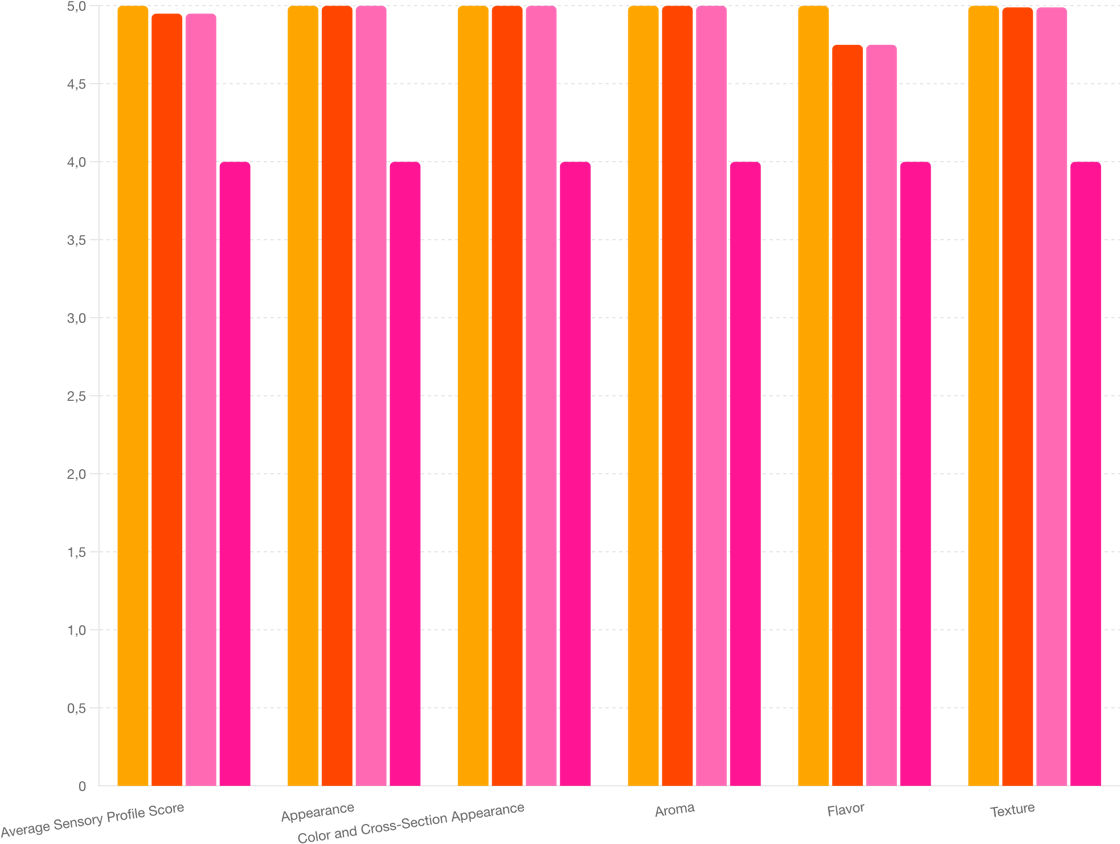
\includegraphics[height=0.4\textwidth, width=\textwidth]{assets/306}
	\caption*{Figure 1 - Sensory analysis of control and experimental sausage
  samples with added purslane}
\end{figure}


\begin{multicols}{2}

The control sausage sample received the highest scores across all
parameters (5.00). Samples with 0.8\% and 1.2\% purslane powder also
received high scores, with negligible differences between them: the
average sensory profile score was 4.95 for both samples. According to
the results of the sensory analysis presented in the chart, the
experimental samples 1 and 2 showed no significant differences from the
control in terms of appearance, color, aroma, and flavor, receiving
scores of 5.00, 5.00, 5.00, and 4.75, respectively. The texture was
slightly lower (4.99) but still at a high level. The sample with 1.4\%
purslane showed a significant deterioration in all sensory
characteristics, including the average score (4.00), appearance (4.00),
color (4.00), aroma (4.00), flavor (4.00), and texture (4.00). These
changes are associated with the emergence of a bitter taste and a
greenish tint in the sausage, significantly affecting its appearance.
Given the minimal differences between the samples with 0.8\% and 1.2\%
purslane, we decided to use experiment 2 with a concentration of 1.2\%
as the primary experiment, as it ensures high sensory scores without
significant changes and provides the best physicochemical properties
described above. Thus, adding 1.2\% purslane to sausages maintains their
quality and improves functional characteristics.

Microbiological safety and food quality are key aspects determining
their suitability for consumption. One of the important indicators used
to assess the microbiological quality of food products, including
sausages, is the total viable count (TVC). This indicator allows for
evaluating the total number of microorganisms capable of growing and
forming colonies under aerobic and facultative anaerobic conditions at
moderate temperatures. In the context of growing demand for organic and
natural products, the use of natural additives to improve
microbiological stability and extend the shelf life of food products is
becoming increasingly relevant. Purslane powder (Portulaca oleracea) is
known for its antioxidant and antimicrobial properties, making it a
promising additive for sausages. This study will help determine the
optimal concentration of purslane powder to achieve the best
microbiological indicators without compromising the organoleptic
properties of the product (Table 2).
\end{multicols}


\begin{longtable}[]{|@{}
  >{\raggedright\arraybackslash}p{(\columnwidth - 10\tabcolsep) * \real{0.1668}}|
  >{\raggedright\arraybackslash}p{(\columnwidth - 10\tabcolsep) * \real{0.0766}}|
  >{\raggedright\arraybackslash}p{(\columnwidth - 10\tabcolsep) * \real{0.1513}}|
  >{\raggedright\arraybackslash}p{(\columnwidth - 10\tabcolsep) * \real{0.1968}}|
  >{\raggedright\arraybackslash}p{(\columnwidth - 10\tabcolsep) * \real{0.2114}}|
  >{\raggedright\arraybackslash}p{(\columnwidth - 10\tabcolsep) * \real{0.1969}}@{}|}
  \caption*{Table 2 - Study of total viable count (TVC) in experimental
  sausage samples} \\
\hline
% \toprule\noalign{}
\begin{minipage}[b]{\linewidth}\raggedright
\vspace{0.7cm}  
Parameter
\end{minipage} & \begin{minipage}[b]{\linewidth}\raggedright
Days
\end{minipage} & \begin{minipage}[b]{\linewidth}\raggedright
Control
\end{minipage} & \begin{minipage}[b]{\linewidth}\raggedright
Experiment 1 (0.8\% purslane)
\end{minipage} & \begin{minipage}[b]{\linewidth}\raggedright
Experiment 2 (1.2\% purslane)
\end{minipage} & \begin{minipage}[b]{\linewidth}\raggedright
Experiment 3 (1.4\% purslane)
\end{minipage} \\
% \midrule\noalign{}
\endhead
% \bottomrule\noalign{}
\endlastfoot
\hline
  
TVC, CFU/g & 1

4

9 & 1,39*10\textsuperscript{2}

1,27*10\textsuperscript{3}

1,43*10\textsuperscript{4} & 1,31*10\textsuperscript{2}

1,47*10\textsuperscript{2}

1,35*10\textsuperscript{3} & 1,11*10\textsuperscript{2}

1,03*10\textsuperscript{2}

1,19*10\textsuperscript{3} & 1,27*10\textsuperscript{2}

1,01*10\textsuperscript{2}

1,05*10\textsuperscript{3} \\
\hline
\end{longtable}

\begin{multicols}{2}

On the first day, all samples showed similar initial levels of TVC, with
slight differences. The lowest number of bacteria was recorded in the
sample with 1.2\% purslane (1.11 × 10² CFU/g). After 4 days, the number
of bacteria significantly increased in the control sample (1.27 × 10³
CFU/g). Samples with the addition of purslane demonstrated much lower
bacterial growth. The sample with 1.4\% purslane showed the lowest
number of bacteria (1.01 × 10² CFU/g), indicating a strong antimicrobial
effect. After 9 days, the control sample showed a significant increase
in bacteria (1.43 × 10⁴ CFU/g), whereas the samples with purslane
maintained lower TVC levels. The sample with 1.4\% purslane again
demonstrated the lowest number of bacteria (1.05 × 10³ CFU/g). The
addition of purslane powder to the sausages significantly reduces the
number of viable bacteria compared to the control sample. The lowest
number of bacteria was recorded in samples with 1.2\% and 1.4\%
purslane, especially on days 4 and 9. Experiment 2 (1.2\% purslane) was
chosen as the primary one since it provides a significant reduction in
bacterial load without noticeable deterioration in the sensory
characteristics of the product. In contrast, Experiment 3 (1.4\%
purslane) imparted a bitter taste and a greenish tint to the sausage,
negatively affecting its appearance and flavor.

{\bfseries Conclusion.} This study demonstrated that adding purslane powder
(Portulaca oleracea) to organic sausages significantly improved their
quality and shelf life. The experimental samples with purslane retained
higher moisture levels and exhibited stable pH values, indicating
enhanced product stability. Water activity remained consistent, ensuring
microbiological safety. The total viable count (TVC) was significantly
lower in samples with purslane, especially at 1.2\% and 1.4\%
concentrations, compared to the control. Sensory analysis revealed that
the sample with 1.2\% purslane had high scores similar to the control,
while 1.4\% purslane negatively impacted flavor and appearance. Organic
beef provided a high-quality protein source without synthetic additives,
aligning with consumer demand for healthier products. Purslane powder,
with its antioxidant and antimicrobial properties, proved to be an
effective natural additive. The use of 1.2\% purslane is recommended,
offering a balance between improved quality and sensory attributes. This
natural approach supports the production of high-quality, organic
sausages without synthetic preservatives.

{\bfseries Gratitude, conflict of interest (financing).} This research is
funded by the Ministry of Science and Higher Education of the Republic
of Kazakhstan (BR21882327)

\end{multicols}


\begin{center}
  {\bfseries References}
  \end{center}


\begin{noparindent}

1.Dkhil M.A., Moneim A.E., Al-Quraishy S., Saleh R. Antioxidant effect
of purslane (Portulaca oleracea) and its mechanism of action // Journal
of Medicinal Plants Research. -- 2011. --Vol. 5. --P. 1589-1593.
https://academicjournals.org/journal/JMPR/article-full-text-pdf/C1D5B4017817\#:\textasciitilde:text=Purslane\%20is\\\%20a\%20potent\%20antioxidant,which\%20act\%20against\%20oxidative\%20stress.

2.Willer H., Lernoud J. The World of Organic Agriculture. Statistics and
Emerging Trends. Research Institute of Organic Agriculture FiBL // IFOAM
Organics International. -2019. ISBN 978-3-03736-119-1

3.Dimitri, C., \& Greene, C. Recent growth patterns in the US organic
foods market // Organic Agriculture. -2016. --Vol. 6(4). --P. 299-310.
DOI 10.22004/ag.econ.33715

4.Esrafil M., Akter S., Alam M., Alim M., Reza M.S., Zubair M.A., Joy
P.R., Jahan M., Khatun M. Development and quality evaluation of novel
biscuits by utilizing fruits and vegetables seed // Food \\Research.
-2024. --Vol. 8(1). --P. 181-189. DOI 10.26656/fr.2017.8(1).090

5.Das S., Raychaudhuri U., Chakraborty R. Herbal fortification of bread
with fennel seeds // Food Technolo-gy and Biotechnology. -2013. --Vol.
51(3). --P. 434-440. https://hrcak.srce.hr/file/160840

6.Petropoulos, S. A., Fernandes, Â., Dias, M. I., Vasilakoglou, I. B.,
Petrotos, K., Barros, L., \& Ferreira, I. C. F. R. Nutritional Value,
Chemical Composition and Cytotoxic Properties of Common Purslane
(Portulaca oleracea L.) // Relation to Harvesting Stage and Plant Part.
In Antioxidants. -2019. --Vol. 8(8). --P. 293-465. DOI
10.3390/antiox8080293

7.Uddin M.K., Juraimi A.S., Hossain M.S., Nahar M.A.A., Ali M.E., Rahman
M.M. (2014). Purslane weed (Portulaca oleracea): a prospective plant
source of nutrition, omega-3 fatty acid, and antioxidant attributes. The
Scientific World Journal, 2014. DOI:10.1155/2014/951019

8. Patarata L., Fernandes L., Silva J.A., Fraqueza M.J. The Risk of Salt
Reduction in Dry-Cured Sausage Assessed by the Influence on Water
Activity and the Survival of Salmonella // Foods. -2022. -Vol.11(30.
-P.444. https://doi.org/10.3390/foods11030444

9. Barbosa-Canovas, G. V., Fontana, A. J., Schmidt, S. J., \& Labuza, T.
P. (Eds.). (2020). Water Activity in Foods: Fundamentals and
Applications/ Wiley.- 616 P. ISBN (electronic)-9781118765982, ISBN
(print- 9781118768316

10.Rashed, A. N., Afifi, F. U., \& Disi, A. M. Simple evaluation of the
wound healing activity of a crude extract of Portulaca oleracea L.
(growing in Jordan) in Mus musculus JVI-1 // Journal of
Ethnopharmacolo-gy.-2003.-Vol. 88(2-3).-P. 131-136. DOI:
10.1016/s0378-8741(03)00194-6
\end{noparindent}

\emph{{\bfseries Information about the authors}}
\begin{noparindent}

K. Makangali - PhD, Kazakh Agrotechnical Research University named after
S.Seifullin, Astana, \\Kazakhstan, e-mail: kmakangali@mail.ru;

G. Ospankulova - candidate of biological sciences, Kazakh Agrotechnical
Research University named after S.Seifullin, Astana, Kazakhstan, e-mail:
bulashevag@mail.ru;;

G. Tokysheva - PhD, Kazakh Agrotechnical Research University named after
S.Seifullin, Astana, \\Kazakhstan, e-mail: tokisheva\_g@mail.ru
\end{noparindent}

\emph{{\bfseries Сведения об авторах}}
\begin{noparindent}

Макангали К.К. - PhD, Казахский агротехнический исследовательский
университет им.С.Сейфуллина, Астана, Казахстан, e-mail:
kmakangali@mail.ru

Оспанкулова Г.Х. - к.б.н., Казахский агротехнический исследовательский
университет \\им.С.Сейфуллина, Астана, Казахстан, e-mail:
bulashevag@mail.ru;

Токышева Г.М. - PhD, Казахский агротехнический исследовательский
университет им.С.Сейфуллина, Астана, Казахстан, e-mail:
tokisheva\_g@mail.ru

\end{noparindent}











